\documentclass{report}
\usepackage{lipsum}
\usepackage{color}
\usepackage{cite}
\usepackage{hyperref}
\usepackage{graphicx}
\newcommand{\hilight}[1]
{\colorbox{yellow}{#1}}
\title{Bringing Bioinformatics to High Schoolers}
\author{Philip Braunstein\\ Advisor: Donna Slonim}
\date{
In Partial Fulfillment of the Requirements for the Degree \\
Master of Science in Computer Science, Tufts University \\
December 2015
}

\begin{document}
\bibliographystyle{apalike}
\maketitle

\chapter*{Acknowledgements}
TBD. Ppl to acknowledge:
Donna, Matt, Mark, Candice, David, Denali, Hannah, Karen (sliding window activity, word-search), Jisoo (Needleman-Wunsch worksheet).  BioSeq, Tufts, Family, Friends,

\tableofcontents

\chapter{Teaching and Curriculum Development}
\section{Overview}
I developed the material for and taught the computer science half of the BioSeq summer course, which was taught in the summers of 2014 and 2015. The BioSeq course is a groundbreaking course that brings bioinformatics to high schools. Rising high school seniors took part in the summer course based on an application process. Students performed wet laboratory work and learned about bioinformatics in the biology section of the course, which was taught by a chemistry postdoc from the Walt Laboratory. The computer science side of this course involved both a lecture component and a practical laboratory component, which are described in the next two sections, respectively. The students performed the wet laboratory work and the analysis for two projects referred to as: Mutations Investigation Experiment and Microbiome Portrait Experiment. 

One of BioSeq's goals is for high school biology teachers to be able use content developed for this course in their classrooms. With this goal in mind, I created powerpoint presentations with all of the course material described below. Some of these materials have been used by BioSeq in their work going into high schools during the year. The teaching resources developed below are located on the BioSeq drive. This is part of the Walt Laboratory shared drive.

\section{Topics Covered}
The computer science section of the BioSeq Summer course covers a range of topics. The students are exposed to information all across the spectrum - the practical instructions to use state of the art bioinformatics tools as well as the theoretical underpinnings of computational biology and computer science. The schedule from the 2015 course is described in some detail below. 

The first topics covered were nucleotide alignment and BLAST  \cite{altschul1990basic}. In this case, BLAST is the practical bioinformatics tool, and nucleotide alignment is the theoretical underpinnings that helps students understand how the practical tool actually works. These topics included INDELs and SNPs, global and local alignment, and scoring schemes for pairwise nucleotide alignment. Students learned about P-Values and E-Values as well as why P-Values are not sufficient for evaluating the significance of BLAST results. 

I believe it is important for bioinformatics students to have cursory knowledge of important topics in computer science theory. With this in mind, the next section of the course consisted of an introduction to information theory (e.g. a question posed to the class is: ``You can quantify length with a ruler, but how can you quantify information?''). Later in the course, I presented other important theoretical computer science topics such as intractability, exponential time complexity, and the traveling salesperson problem (TSP). Furthermore, students learned fundamental classes of algorithms: greedy algorithms, dynamic programming algorithms, and brute-force algorithms. 

Multiple sequence alignment and CLUSTAL Omega \cite{sievers2011fast} were taught as the next iteration of pairing practical bioinformatics tools with theoretical underpinnings. In order to teach multiple sequence alignment, the students were also introduced to the concepts of trees and graphs.

The hardest section of the course covered the Needleman-Wunsch Algorithm \cite{needleman1970general} for global pairwise nucleotide alignment. The students ran example problems by hand using this dynamic programming algorithm. Students filled out the matrix as well as performed the traceback to determine the correct alignment from the matrix. This included finding all best-scoring alignments when there were more than one best-scoring alignment. This material is typically only taught to computer science major upperclassmen at universities and computer science graduate students, and it was an excellent opportunity for these high school students to understand how a real and relevant algorithm works. Students also saw that it takes very minimal modifications to adapt this algorithm for local alignment (the Smith-Waterman Algorithm \cite{smith1981identification}).

I taught different approaches to constructing next-generation sequencing experiments - in particular the difference in approach between using \emph{de novo} and resequencing approaches. I also introduced students to more specialized versions of sequencing such as RNA-Seq \cite{nagalakshmi2008transcriptional} and ChIP-Seq \cite{johnson2007genome}. Through this section of the course, students learned that the effects of next-generation sequencing are broader than at first anticipated. In this section of the course, the students learned the theoretical underpinnings of how Sanger Sequencing \cite{sanger1977dna} works.

As a final subject in the computer science half of the BioSeq Summer Course 2015, I taught metagenomics experiments. I presented two main classes of metagenomics experiments: targeted 16S sequencing \cite{qin2010human} and whole genome shotgun (WGS) sequencing \cite{chen2005bioinformatics}. Students learned the different information that these variants of metagenomics experiments evince. We studied (and in the computer science lab, used) software called PICRUSt \cite{langille2013predictive} that converts 16S reads into predicted WGS reads. 

\section{Computer Science Labs}
The computer science side of the BioSeq course also had a computer science laboratory component. I developed a number of labs to be used in conjunction with the Summer Course. These labs were mostly developed in the academic year leading up to Summer 2015 - for the first summer that the course was taught, I used labs from a bioinformatics textbook. While these textbook labs were sufficient, it was important for BioSeq to develop its own computer science lab content. This insures that it can exported for use by high school teachers.


\subsection{Global and Local Alignment}
The goal of the first lab is to give students practical experience working with alignment software as well as teach them the differences between local and global alignment. Students learn in which situations it is relevant to use each of these alignments techniques. Students also become familiar with FASTA file formats in this lab, and they use EMBOSS NEEDLE for global alignment and EMBOSS WATER for local alignment \cite{rice2000emboss}.

The students use global alignment to align human and mouse homologs of the RNA for MTOR (\textbf{M}echanistic \textbf{T}arget \textbf{o}f \textbf{R}apamycin). They use local alignment to align the complete CDS of human P53 to a particular transcript variant of P53. This second alignment illustrates a problem in which local alignment is a better choice than global alignment. This is because the complete CDS is much longer than the spliced transcript. Global alignment would unnecessarily penalize the different sizes of the sequences. 

\subsection{BLAST}
The BLAST lab gives students practical experience working with BLAST - one of the most important, most used tools in the field of bioinformatics. Students learn how to use the statistics from BLAST including E-Value, percent identity, and query cover. Students also get practice manipulating advanced settings of BLAST (namely, which databases and/or organisms to search).

In the BLAST lab, students use the human DNA sequence for IMPDH2 (\textbf{I}nosine 5'-\textbf{M}ono\textbf{p}hosphate \textbf{D}e\textbf{h}ydrogenase \textbf{2}) to search the DNA databases of other organisms to identify the homologs in these species.

\subsection{Multiple Sequence Alignment}
In this lab, students use CLUSTAL Omega to perform multiple sequence alignment of the Hexokinase gene RNA from human, mouse, chicken, frog, and plant in order to build a phylogenetic tree. This lab also prompts students to think about some of the biological consequences of the selection of Hexokinase as the gene used for the alignment (``Would you hypothesize that hexokinase is an essential gene for all the organisms?'' ``Why would dystrophin not have been a good gene to use for this lab [dystrophin is only found in mammals]?'').


\subsection{Mutations Investigations Experiment Analysis}
The Mutations Investigation Experiment (MIE) is a blue-white screen on bacteria susceptible to mutation. The automated analysis from the MiSeq used by BioSeq reports the location and identity of mutations in the plasmid DNA in the bacteria, but it does not extrapolate to show what changes in the Lacz-$\alpha$ peptide have occurred on account of these mutations. Students each look at a white colony (contains a mutation that disables LACZ) and a blue colony (functional LACZ) to see if they can come up with a hypothesis, of why the white colony turned white (i.e. what mutated within the bacteria such that it could no longer produce functional Lacz protein?).

The MIE computer science lab introduces students to the concept of \emph{in silico} translation to see the effects of the mutations in the plasmid DNA. The students also look at other susceptible parts of the plasmid that don't get translated into protein (promoter, origin of replication, etc.) to see if a mutation in these areas could explain a colony's white color.

\subsection{Microbiome Portrait Experiment Analysis}
In the microbiome experiment, students each swab their retroauricular crease (behind the ear) and hard palate in order to sequence the microbiomes living in these regions. The students use PICRUSt to generate the predicted WGS reads from the 16S sequencing results. The students then use LEfSe \cite{segata2011metagenomic} to find functions statistically enriched at each of these areas. Discussion questions help students come up with reasons why certain functions would be enriched in one of these regions (in comparison to the other). The analysis also seeks to answer whether samples closer by individual or by sample location. This section of the lab is answered by students running part of the analysis code described below.

\subsection{Fastq Knowledge}
\noindent This lab was never run with BioSeq students. It provides a UNIX command line interface through which students can interact with FASTQ files to help them understand the information contained within - regardless of the students' programming background.

Fastq Knowledge reads in a FASTQ file, and prompts the student (through the command line) to select the information that the student wants to know about the file. Supported questions include querying the number of each type of nucleotide in the file, the GC content, the number of pages it would take to print the file in 12-point font, etc. See the corresponding figure regarding this lab.

\begin{figure}[h]
\centering
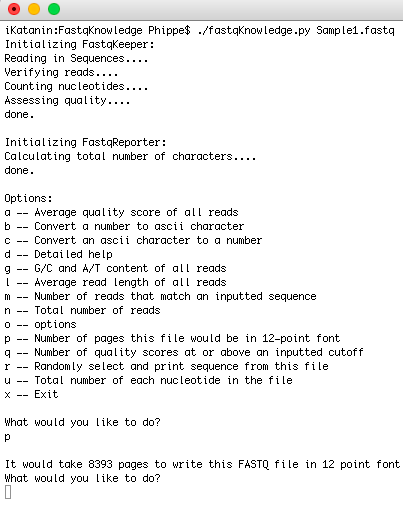
\includegraphics[scale=0.75]{fastqK.png}
\caption{Fastq Knowledge in action}
\end{figure}


\section{Classroom Activities}
The classroom activities I developed for BioSeq are described below. Some of these were assigned as homework assignments during the course. These are all documented on the BioSeq shared drive.

\subsection{Sliding Window Activity}
Karen O'Hagen suggested this idea: A folded piece of paper with a window cut into it allows the user to see sequence written on one of two inserts provided with the activity. There is a sequence printed on the front of the folded piece of paper, and the students attempt to align the sequence on each insert to the sequence on the front of the paper. One of the sequences on the inserts has a gap and one does not - only the gapped insert aligns well. This activity is designed to show students why it is important to be able to insert gaps during sequence alignment as well as introduce them to the complexity of the sequence alignment problem.

\subsection{Alignment Worksheets}
I developed several generations of nucleotide alignment worksheets to help students practice pairwise nucleotide alignment. In these worksheets, the reference is fixed, and the students write the corresponding read underneath each reference. Students have the option of inserting gaps into the reads they write. However, it is impossible for students to insert gaps into the reference because it is printed onto the page.

\subsection{Sanger Sequencing Worksheet}
Denali and I developed a worksheet to teach Sanger sequencing. Students deduce the sequence of a nucleotide sequence by reading an illustration of a Sanger sequencing gel.

\subsection{Graph Drawing}
In order to familiarize students with graphs, I call students up to the board by birthday. All January birthdays write their first names in a node on a graph, and every January birthday adds an edge to every other January birthday. This process is repeated for each month of the year, and at the end, the students have created a graph representation of the birthdays in the classroom.

\subsection{Protein Alignment Worksheet}
Hannah and I developed a worksheet for protein alignment using the BLOSUM-62 similarity matrix \cite{henikoff1992amino}.

\subsection{Paired-End Sequencing Quotations Activity}
This activity gives students an intuitive idea for how paired-end sequencing works \cite{roach1995pairwise, fleischmann1995whole}. This activity was developed in conjunction with Denali. We selected famous quotations from biology and computer science (e.g. ``The biggest difference between time and space is you can't reuse time''), and we split each quotation in half and gave each half of the quotation the same marking, for example, an orange star. We selected a total of 10 or 20 quotations and prepared them in this way. The quotations are passed out at random to the students, and each students had to find his or her ``mate-pair'' to complete the quotation. Afterwards, each pair of students reads their quotation aloud.

\subsection{Coverage Word-Search}
This activity helps students acquire an intuitive idea of what the concept of coverage means. Karen O'Hagen suggested this idea: I created a word search with bioinformatics vocabulary; however, some of the words are repeated more than others. For example, the word ``bit" is in the word search twice, while the word ``coverage'' is in the word-search eight times. In this example, the words that show up more in the word search have the higher coverage.

\subsection{Sorting Hat Assembly Song}
Hannah and I developed an activity to help students understand \emph{de novo} sequencing assembly. We obtained the words from the Sorting Hat Song from the first Harry Potter and the Philosopher's Stone \cite{rowling1997harry} , and we split the song into reads, such that there was some overlap between the reads. The students are asked to assemble the reads on the floor of the classroom. Once complete,  one of the students is asked to recite the assembled song. We chose the Sorting Hat Song because most students will be familiar with it, but it is long and complicated enough that it is unlikely that students will have the entire song memorized. 

\subsection{Sequencing Techniques Worksheet}
Hannah and I developed this worksheet which helps students recognize in which situations it is appropriate to use different sequencing techniques. A number of experimental goals are provided in the setup, and the students must decide whether to use \emph{de novo} sequencing, resequencing, microbiome sequencing, RNA-Seq, or ChIP-Seq.

\subsection{16S Microbiome Analysis Activity}
The standard analysis of 16S microbiome sequence clusters reads of greater than or equal to 97\% sequence similarity as coming from the same bacterium \cite{glockner2000comparative}. In order to help students understand this analysis strategy, Hannah and I developed an activity in which there are three categories of names: for example, Maria, Bob, and Sandy. There are a number of reads, each of which fits one of these name categories best. For example, ``Mandy'' belongs in the Sandy family of names, and ``Blob'' belongs in the Bob family of names. Students must categories all of the input names they are given.

Furthermore, each name has a set of foods that s/he likes to eat in order to introduce the idea of functions within a microbiome community. For example, Sandy can eat ten pieces of pizzas and one ice cream. Bob can not eat pizza, but he can eat seven ice creams. Students can then talk about the capabilities of each community as a whole. Conversations guided in the classroom have the following tenor, "Community A has a lot of Sandy-family names, so this community is good at eating pizza and not that good at eating ice cream." Note that this process of designating community function based on the food each name likes is almost exactly analogous to how PICRUSt converts 16S reads to WGS reads (see above).


\chapter{Development of Analysis Code}
\section{Overview}
I wrote most of the code for the analysis used by the BioSeq group. These analyses can be found on the BioSeq Group's Github Account. The majority of the analysis code is written in Python, and there are small written components in other languages (notably R). Please see the Github repo for each project for more extensive documentation.

\section{Genetics of Race}
\url{https://github.com/BioSeq/Genetics-of-Race-Analysis} \\

\noindent In the Genetics of Race experiment, students have two hyper-variable regions (HVR) of their mitochondrial DNA sequenced. At the end of the experiment, each student receives the name of the other student in the class, with whom s/he is most genetically similar to according to their mitochondrial DNA. 

The Genetics of Race Analysis takes as input VCF files generated by the MiSeq (a read aligner and GATK are part of the MiSeq's built-in workflow - these generate the VCF files) as well as the FASTA files of the reference sequence of the two hyper-variable regions sequenced. The Genetics of Race Analysis uses the reference files as well as the VCF files from each student to generate a FASTA file containing the sequences that \emph{would have been seen} in each of the student's mitochondrial DNA (i.e. the variants from the VCF file are incorporated into the reference sequence to generate the sequence seen in each student's mitochondrial DNA). The output of the script is a FASTA file, wherein each entry is one student's reconstructed HVRI and HVRII sequence concatenated together.

CLUSTAL Omega can be used to generate a phylogenetic tree and a matrix of the students' similarities to one another from this output file, which is used to inform each student of the other student in the class, with whom s/he shares the greatest similarity based on mitochondrial DNA sequence.

There have been three generations of the Genetics of Race Analysis code. The first version was a shell script that became insufficient once the sample-indexing used by the BioSeq wet laboratory scientists changed. The second version was a Python script that depended heavily on the Broad Institute's GATK  \cite{mckenna2010genome}. The current version of the analysis is no longer dependent on GATK; this became necessary once we became interested in developing Mac OS X and Windows apps for the Genetics of Race Analysis (see below).

\section{Metagenomics Analysis}
\url{https://github.com/BioSeq/Metgenomics-Analysis}\\

\noindent In the Metagenomics experiment, students sequence the microbiomes living on their hard palate (HP) and retroauricular crease (RA) (behind the ear). One goal of this experiment is to see whether microbiome similarity clusters by individual or by body-site. In other words, is it more likely that student X's HP microbiome will be most similar to student X's RA microbiome or to student Y's HP microbiome.

The \texttt{run.py} script coordinates all of the analysis for the metagenomics analysis so that the user only needs to run one script to generate all of the results. Every time the \texttt{run.py} is run, a unique UUID is generated so that all of the output files from each run can easily be grouped together. This script executes all of the other scripts in the Metagenomics Analysis program as subprocesses.

The Metagenomics Analysis generates an OTU table that can be used for the PICRUSt lab described above as well as a phylogenetic tree of the all of the samples labeled by student and by bodysite. This tree clearly shows whether the metagenomes cluster by person or by body site for each run. 

This program also randomly shuffles and reassigns the student IDs used by the BioSeq wet lab scientists. This provides a double-blind style of information security, in which nobody can fully identify a student's position in the tree (not even BioSeq employees). 

\begin{figure}[h]
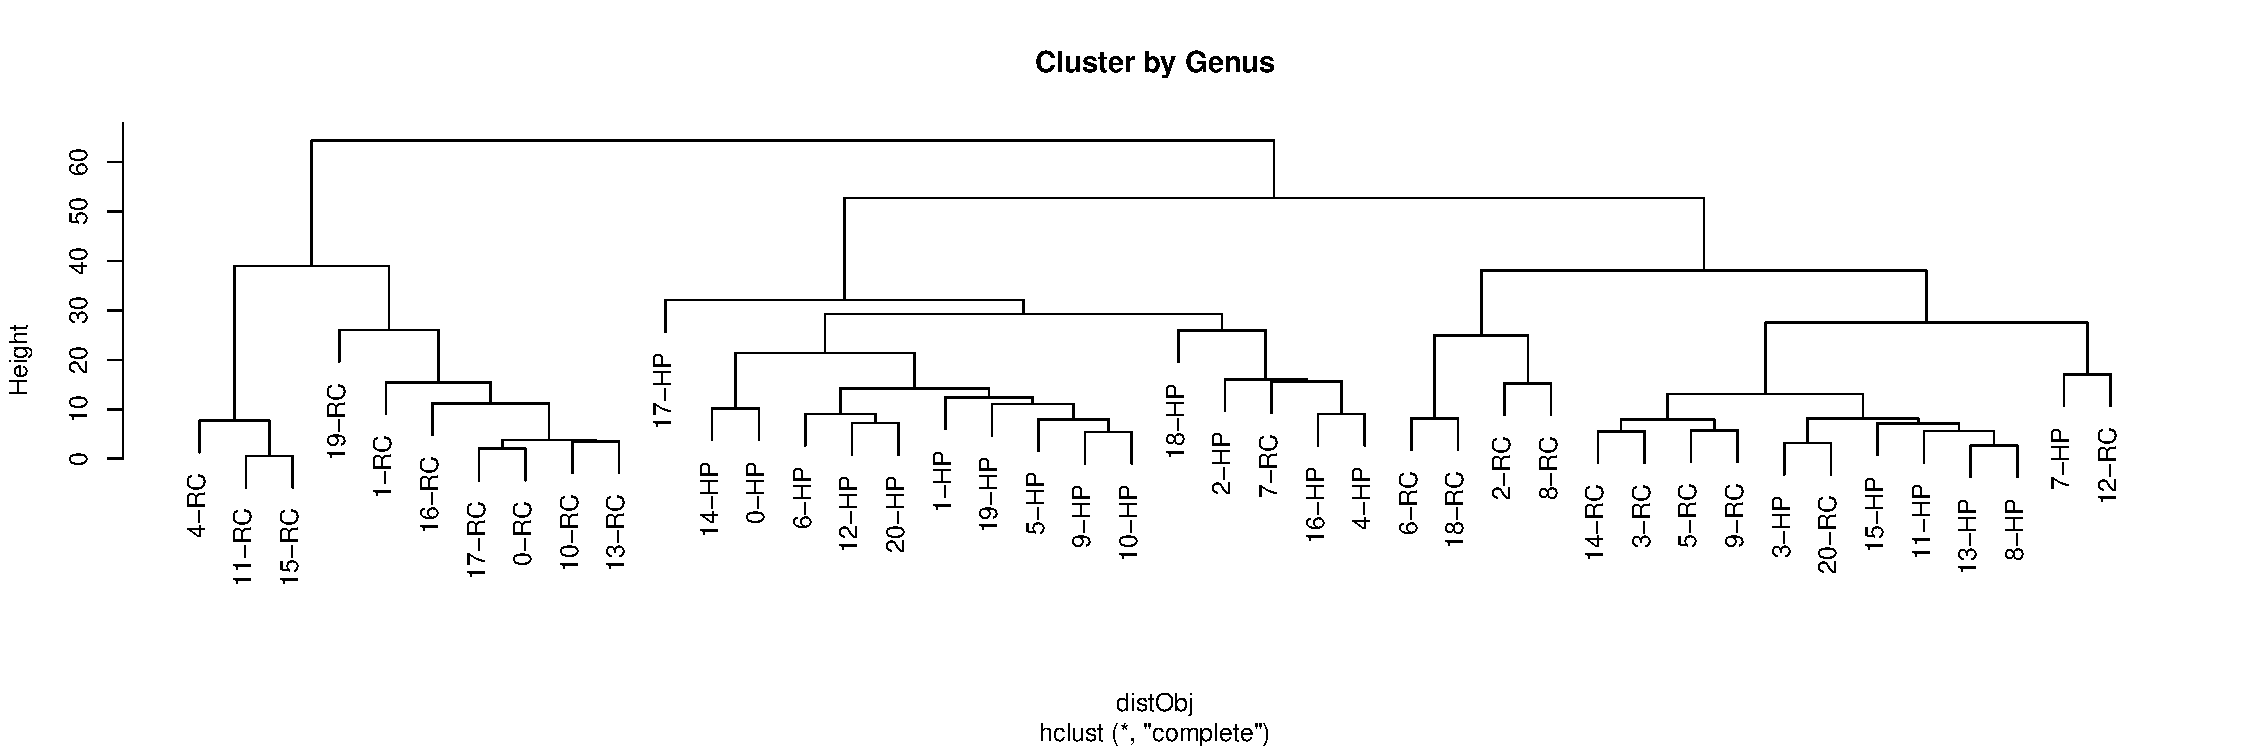
\includegraphics[width=\linewidth]{tree.pdf}
\caption{Clustered metagenomic samples. The number refers to (randomized) student's ID and HP and RC refer to hard palate samples and retroauricular crease samples respectively}
\end{figure}

\section{Mac OS X and Windows Desktop App for Genetics of Race}

I built Mac OS X and Windows desktop apps for the Genetics of Race analysis. The goal of this is to enable teachers with no computer science experience to be able to run the Genetics of Race analysis themselves. This project involved building a simple front-end with Python's Tkinter \cite{shipman2005tkinter}. 

The Mac app uses py2app (\url{https://pythonhosted.org/py2app/}) to bundle the Genetics of Race script, a Python interpreter, and data files into a Mac OS X executable. The program pyinstaller (\url{http://www.pyinstaller.org/}) is used to turn the script into a Windows exe file. Due to differences in how Mac and Windows handle creating executable files, it was not possible to include the FASTA sequence reference supporting files in the Windows exe install. To circumvent this problem, I saved the hyper-variable sequences as string constants within the python script for the Windows build. Within the Mac build, these sequences are stored in FASTA files that are read by the Python script. 

Both Mac and Windows apps contain a compile script written as a shell script and as a batch script, respectively. These scripts clean up the previous build and launch the next build. The shell script for the Mac app also moves the FASTA files to the appropriate place within the app so that the script can access them.


\chapter{Mentorship}
\section{Overview}
As the graduate student from computer science, I spent some of my time working in BioSeq mentoring other BioSeq members with ideas and techniques from  bioinformatics and computer science. 

\section{Website development}
In the summer of 2014, I oversaw the development of the BioSeq webpage (\url{http://ase.tufts.edu/chemistry/walt/sepa/index.html}) by Denali Rao, who is a computer science undergraduate student at Tufts. Working with Denali was my first experience with management, and I learned much from this experience. Throughout the process I suggested some potential frameworks and designs to use, but I found giving her the space to make her own decisions led to a better final product. In addition, the more Denali accomplished on her own (rather than implementing what I had dictated), the happier she seemed to be with her work and the easier my job as a manager was.

Denali chose to use the Bootstrap CSS framework (\url{http://getbootstrap.com/}) to make the webpage. She was particularly interested in this framework because it works well with responsive web, and it runs on different size screens with no adjustments necessary. We iterated through a couple of different designs of the webpage, finally ending up at the website currently in production.

\section{Introduction to Programming Course for Undergraduate BioSeqers}
\subsection{Overview}
In the summer of 2014, I ran a programming seminar for the undergraduate students working for BioSeq. These students were primarily majoring in the biological sciences and had little to no previous experience with computer science. To start with, I had the students do the Python Codecademy Python track (\url{https://www.codecademy.com/learn/python}) in order for them to learn the syntax and use of Python. After a demo, in which I demonstrated how to solve a complicated problem with programming, students completed five programming assignments described below. All assignments are available on the BioSeq shared drive.

\subsection{Demo}
Codecademy is an effective teaching tool for introducing students to features and syntax of the language; however, it does not show students how to solve complicated problems with programming. I demoed solving a complicated problem with a Python script.

The inputs to this demo were two files: one containing a list of countries by continent and another containing list of the GDP of various countries in 2004 and 2012. The goal was to write a program to calculate change in GDP from 2004 to 2012 by continent. This was a good demo project because it is simple enough that it can be solved within an hour with a single Python script. However, the problem is not trivially solvable, and important choices need to made.

\subsection{a1}
Given a codon table in the form of a text file, students write a program that translates a nucleotide sequence to an amino acid sequence provided on the command line by the user. Students are instructed to only translate the nucleotide string in the first of the six reading frames.

Students are exposed to some basic error handling in this assignment. They decide how to handle sequences that are not a multiple of three (the most natural solution is to remove the last one or two remaining nucleotides in this case). They also must handle sequences containing non-nucleotide characters (`D', for example).

One twist in the assignment is the codon table is saved is formatted as follows: the first column of each row is an amino acid, and the rest of the columns in that row are the codons that code for the amino acid in the first column. This is tricky for two reasons. First, not every row has the same number of columns (because some amino acids have more corresponding codons). Second, this organization of the table is not as intuitive for translation because translation involves reading a codon and translating it into an amino acid. Excellent submissions took this into account and did some extra work while reading the file so that the codon dictionary was structured with the codons as keys and the amino acids as the values. This is the best metaphor for what actually happens when translation occurs in the cell. This is in contrast to the dictionary the students created when reading in the file naively: amino acids as keys and a list of nucleotides for each value.

\subsection{a2}
Given a gene table from UCSC \cite{karolchik2003ucsc} of a certain format (described in more detail in the assignment), students write a program to read the table and output a new table with the genes in descending order of CDS length. In addition, only genes with at least ten exons should be written to the new file. 

This is the students' first experience dealing with data that is big enough such that it is impossible to look at every line by hand. Bioinformatics is a field of big data, so it is imperative for students to be comfortable dealing with sizable data.

This assignment also lends itself well to a discussion of the value of programming with constants. When students use constants in this script, it becomes easy to modify the script for different requirements. A single constant at the top of the file with the exon-number-cutoff, makes it exceedingly easy to modify the program so that it writes out all genes with three or more exons -- or any arbitrary number.

\subsection{a3}
Students write a program that takes a FASTQ file and a sequence on the command line. The program reads through the FASQ file and prints the number of reads that contain the sequence provided to the program.

Through this assignment, students learn how to process an input file, in which not all of the lines are relevant. Each FASTQ entry has four lines, and only the second line is useful for completing this assignment. Furthermore, FASTQ files are a staple of bioinformatics, and it is important for students to get experience working with them.

\subsection{a4}
This assignment is an extension of a3. The students modify their submissions for a3 so that the program takes one extra command line argument: an ascii character referring to the quality score of each read. Illumina sequencing platforms use a clever ascii code system to indicate the quality of each nucleotide of each read read. A detailed discussion of Illumina quality scores is beyond the scope of this document, but the reader can find a more information in the citations \cite{cock2010sanger}.

In a limited capacity, this assignment introduces the students to the concept of needing to be able to maintain and extend code they write.

\subsection{a5}
This last project serves as the final project for this programming course. In this project, students implement the dynamic programming Needleman-Wunsch Algorithm for pairwise global sequence alignment. This is a complicated project, and I evaluate it as being a similar difficulty as the final project from the first semester of computer science at Tufts University.

This program requires students to grapple with recursive function calls as well as programming with matrices. In the Needleman-Wunsch Algorithm, a matrix is constructed, and it is necessary to traverse this matrix recursively in the traceback section of the algorithm in order to find the best scoring alignment. In addition, if there exists more than one equally best scoring alignment, the algorithm (and thus the program) must report all of the best scoring alignments. This requires one recursive call of the traceback function sometimes spawning \emph{more than one} follow-up recursive calls.


\section{Professional Development Material for BioSeq Members}
\subsection{Overview}
In the summer of 2015, I lead a three day professional development seminar for the BioSeq members. This was designed to teach BioSeq members basics of the computer science side of bioinformatics. This professional development seminar included interactive components for the participants to use their computers to get practice using the tools described in the presentation.

\subsection{How to Get Data and How to Store It}
This presentation introduced the BioSeq employees to common sources of data and commons means to store data. The presentation described such general topics as whether a flat file is sufficient to store data or a database is necessary, the differences between human-readable files and binary files, and the concept and use of accession numbers in databases.

This presentation introduced a number of common bioinformatics databases including activities for some of them for the employees watching the presentation to get practical experience searching through the databases. It covered NCBI (\url{http://www.ncbi.nlm.nih.gov/}), GEO \cite{edgar2002gene}, Genome Browsers (specifically UCSC), GO \cite{ashburner2000gene}, PDB \cite{berman2000protein}, UniProt \cite{apweiler2004uniprot}, STRING \cite{von2003string}, and KEGG \cite{ogata1999kegg} databases. In conjunction it covered use of SRA-Toolkit \cite{leinonen2010sequence} to extract FASTQ files from downloaded SRA files.

\subsection{Bioinformatics Tools}
This presentation started with a discussion of sequence alignment in bioinformatics. This included SNPs and INDELs, alignment scoring systems, the difference between global and local alignment, the difference between nucleotide and protein alignment, and protein substitution matrices (BLOSUM-62). There was also practical information in these slides regarding the sequence alignment programs BLAST (types BLASTN BLASTP, and BLASTX) as well as CLUSTAL Omega.

A number of other common bioinformatics tools were presented here: online interfaces for bioinformatics tools such as Galaxy (\url{https://usegalaxy.org/}) and SDSC Biology Workbench (\url{http://workbench.sdsc.edu/}); RNA-Seq tools such as Bowtie2 \cite{langmead2012fast}, BWA \cite{li2009fast}, Tophat \cite{trapnell2009tophat}, Cufflinks \cite{trapnell2012differential}, Samtools \cite{li2009sequence}, and GATK; microbiome analysis tools such as QIIME \cite{caporaso2010qiime}, MOTHUR \cite{schloss2009introducing}, and PICRUSt; finally common file types such as FASTA, FASTQ, SAM, BAM, BED, and VCF.

\subsection{Resources at Tufts and Introduction to the Command Line}
The final presentation in this series described practical resources at Tufts that are useful for computing. This included linux accounts with the computer science department, accounts with the research compute cluster, and hints for installing software (local vs. global). This presentation also included an introduction to interacting with the command line on a linux system (the computer science department uses a Redhat distribution). This included standard UNIX commands such as \texttt{pwd}, \texttt{mv}, \texttt{ls}, etc.


\chapter{Development of Computer Science-Only Module}
\section{Overview}
BioSeq develops next-generation sequencing educational modules that are used during the summer course as well as in  Massachusetts high schools throughout the year. The Genetics of Race and Metagenomics modules described above are examples. In most current modules, student interact much more with the wet-laboratory side of bioinformatics than the computer science side of the discipline. The goal of this computer science-only module (that is, no wet-laboratory work involved) is to give students experience analyzing bioinformatics data. The analysis requires several steps and involves several different bioinformatics software packages. The goal is for students to see the computer science part of bioinformatics as more than just a blackbox.

\section{Setup}
The problem will be presented to the students as follows: a biology group ran an RNA-Seq experiment, but they don't know how to analyze the data. This biology group is contracting the students to do the analysis for them. 

The data used in this experiment comes from the SRF-knockout paper published in Blood: SRF is required for neutrophil migration in response to inflammation \cite{taylor2014srf}. The paper contains a relatively simple setup of a wild-type sample and an SRF knock-out sample - each with two biological replicates.

The students use the main galaxy instance to do all of the analysis. This extraordinary tool allows the students to run complicated RNA-Seq analysis all through an easy to use graphical interface.

\section{Procedure}
\subsection{Obtaining the Data}
The data can be download from GEO with accession number GSE55090. It must be downloaded in the form of SRA files which can be converted to FASTQ files using SRA-Toolkit. This step should be done before the students start working with the data since it requires using the command line SRA-Toolkit.

\subsection{Creating a Galaxy Account and Uploading the Data}
The data is big enough such that it needs to be uploaded by an FTP client. There are a number of free and easy to use FTP clients available for the Windows, Mac, and Linux operating systems. 

Galaxy unfortunately uploads data using the insecure FTP protocol instead of the secure sFTP protocol. The consequence of this is that the username and password are transferred to the Galaxy servers unencrypted in plaintext. This means that anyone using the same wifi connection can see the username and password \emph{with almost no effort}. Therefore, it is very important for teachers to instruct their students to choose a password that is not used \emph{with any of their other accounts on the internet}. 

Students should upload the SRR1171332.fastq and the SRR1171334.fastq files, which are one biological replicate each of the WT and KO samples, respectively.

\subsection{Formatting the Data}
After uploading to the file to Galaxy, run the \texttt{FASTQ Groomer} program that can be found under the NGS:QC and manipulation tab. This function must be used with default settings on both of the uploaded FASTQ files,  

\subsection{Aligning the Reads}
Align the reads from each of the files to the mm10 genome. Use the default settings with the built in mm10 reference genome with the \texttt{Tophat} program. This can be found under the NGS: RNA-Seq tab.

\subsection{Assembling Transcripts}
Assemble the transcripts using the \texttt{Cufflinks} program found under the NGS: RNA-Seq tab in galaxy. Use the default settings of Cufflinks on each of the accepted hits files from the mapping step.

\subsection{Comparing}
Run \texttt{Cuffmerge}, which can be found under the NGS:RNA-Seq tab on galaxy on the assembled transcripts files from the Cufflinks step. Use default settings. The output of this step should be used as the input for \texttt{Cuffdiff} program to calculate the differences in expression between the two samples. 

\bibliography{thesis}



\end{document}